%(BEGIN_QUESTION)
% Copyright 2009, Tony R. Kuphaldt, released under the Creative Commons Attribution License (v 1.0)
% This means you may do almost anything with this work of mine, so long as you give me proper credit

Compare the behaviors of these three conductivity probes to a steadily increasing liquid conductivity over time, noting whether the meter indication {\it increases}, {\it decreases}, or {\it remains the same} as the liquid's conductivity steadily increases:

$$\includegraphics[width=15.5cm]{i04128x01.eps}$$

% No blank lines allowed between lines of an \halign structure!
% I use comments (%) instead, so that TeX doesn't choke.

$$\vbox{\offinterlineskip
\halign{\strut
\vrule \quad\hfil # \ \hfil & 
\vrule \quad\hfil # \ \hfil \vrule \cr
\noalign{\hrule}
%
% First row
{\bf Probe design} & {\bf Meter indication} \cr
%
\noalign{\hrule}
%
% Another row
Two-electrode (ammeter) &   \cr
%
\noalign{\hrule}
%
% Another row
Two-electrode (voltmeter) &   \cr
%
\noalign{\hrule}
%
% Another row
Four-electrode &   \cr
%
\noalign{\hrule}
%
% Another row
Electrodeless &   \cr
%
\noalign{\hrule}
} % End of \halign 
}$$ % End of \vbox

Be prepared to explain {\it why} each meter's indication changes as it does!

\vskip 10pt

Now, determine how the meter's indication will be affected by a steady accumulation of residue (``plating'') on the probes over time, identifying whether the meter indication will {\it increase}, {\it decrease}, or {\it remain the same}:

% No blank lines allowed between lines of an \halign structure!
% I use comments (%) instead, so that TeX doesn't choke.

$$\vbox{\offinterlineskip
\halign{\strut
\vrule \quad\hfil # \ \hfil & 
\vrule \quad\hfil # \ \hfil \vrule \cr
\noalign{\hrule}
%
% First row
{\bf Probe design} & {\bf Meter indication} \cr
%
\noalign{\hrule}
%
% Another row
Two-electrode (ammeter) &   \cr
%
\noalign{\hrule}
%
% Another row
Two-electrode (voltmeter) &   \cr
%
\noalign{\hrule}
%
% Another row
Four-electrode &   \cr
%
\noalign{\hrule}
%
% Another row
Electrodeless &   \cr
%
\noalign{\hrule}
} % End of \halign 
}$$ % End of \vbox


\vskip 20pt \vbox{\hrule \hbox{\strut \vrule{} {\bf Suggestions for Socratic discussion} \vrule} \hrule}

\begin{itemize}
\item{} Explain why we use a {\it voltage source} in the ``ammeter'' style of two-electrode cell, and a {\it current source} in the ``voltmeter'' style of two-electrode cell.  What would happen if we mixed up the meter and source styles (e.g. ammeter with a current source; voltmeter with a voltage source)?
\item{} Is it possible to use an AC excitation source rather than a DC source in either the 2-electrode or 4-electrode cell designs?  Explain why or why not.
\item{} Is it possible to use a DC excitation source rather than an AC source in the electrodeless cell design?  Explain why or why not.
\item{} Identify something we could do to the liquid solution to increase its conductivity.
\item{} Identify something we could do to the liquid solution to decrease its conductivity.
\end{itemize}

\underbar{file i04128}
%(END_QUESTION)





%(BEGIN_ANSWER)


%(END_ANSWER)





%(BEGIN_NOTES)

Effect of steadily increasing conductivity over time:

% No blank lines allowed between lines of an \halign structure!
% I use comments (%) instead, so that TeX doesn't choke.

$$\vbox{\offinterlineskip
\halign{\strut
\vrule \quad\hfil # \ \hfil & 
\vrule \quad\hfil # \ \hfil \vrule \cr
\noalign{\hrule}
%
% First row
{\bf Probe design} & {\bf Meter indication} \cr
%
\noalign{\hrule}
%
% Another row
Two-electrode (ammeter) & increases \cr
%
\noalign{\hrule}
%
% Another row
Two-electrode (voltmeter) & decreases \cr
%
\noalign{\hrule}
%
% Another row
Four-electrode & decreases \cr
%
\noalign{\hrule}
%
% Another row
Electrodeless & increases \cr
%
\noalign{\hrule}
} % End of \halign 
}$$ % End of \vbox

\vskip 10pt

Effect of steadily increasing plating over time:

% No blank lines allowed between lines of an \halign structure!
% I use comments (%) instead, so that TeX doesn't choke.

$$\vbox{\offinterlineskip
\halign{\strut
\vrule \quad\hfil # \ \hfil & 
\vrule \quad\hfil # \ \hfil \vrule \cr
\noalign{\hrule}
%
% First row
{\bf Probe design} & {\bf Meter indication} \cr
%
\noalign{\hrule}
%
% Another row
Two-electrode (ammeter) & decreases \cr
%
\noalign{\hrule}
%
% Another row
Two-electrode (voltmeter) & increases \cr
%
\noalign{\hrule}
%
% Another row
Four-electrode & remains the same \cr
%
\noalign{\hrule}
%
% Another row
Electrodeless & remains the same \cr
%
\noalign{\hrule}
} % End of \halign 
}$$ % End of \vbox


%INDEX% Measurement, analytical: conductivity

%(END_NOTES)


